\documentclass[10pt,a4paper]{article}

\usepackage[T1]{fontenc}
\usepackage[utf8]{inputenc}
\usepackage[romanian]{babel}
\usepackage{times}
\usepackage{graphicx}
\usepackage{array}
\usepackage{amssymb}
\usepackage{hyperref}
\usepackage{enumitem}
\usepackage{geometry}

\geometry{
    a4paper,
    left=1.35cm,
    right=1.35cm,
    top=1.25cm,
    bottom=1.25cm
}

\setlength{\parindent}{0pt}
\setlength{\parskip}{0.18em}
\setlist{nosep,leftmargin=*}
\renewcommand{\arraystretch}{1.12}
\pagestyle{empty}

\begin{document}

\begin{center}
    {\Large\bfseries TOOL COLABORATIV SEMI-AUTOMAT DE}\\[-1pt]
    {\Large\bfseries ADNOTARE}\\[-1pt]
    {\small Student: Grigoras Victor-Andrei}
\end{center}

\section*{Introducere}

Adnotarea imaginilor este o etapă esențială pentru construirea seturilor de date folosite în detecție, segmentare și evaluare vizuală. Procesul devine costisitor atunci când obiectele au contururi complexe, când este nevoie de corecții repetate sau când mai mulți utilizatori trebuie să lucreze pe aceeași imagine. Proiectul PyVisionAnnotator propune un instrument desktop care păstrează controlul manual al utilizatorului, dar introduce asistență automată prin modele de segmentare și detecție, inclusiv YOLOE~\cite{yoloe} pentru AutoSeg și Mask2Former~\cite{mask2former} pentru generarea de măști, în raport cu instrumente consacrate precum CVAT~\cite{cvat} și LabelMe~\cite{labelme}.

\section*{Obiective}

\begin{center}
\small
\begin{tabular}{|p{0.96\textwidth}|}
    \hline
    Oferirea unui flux de adnotare manuală pentru dreptunghiuri, poligoane și măști. \\
    \hline
    Integrarea unor mecanisme AI pentru pre-adnotare și pentru generarea rapidă de măști. \\
    \hline
    Susținerea lucrului colaborativ prin autentificare, sesiuni partajate și chat. \\
    \hline
    Exportul datelor în formate utile pentru dataseturi și fluxuri de antrenare. \\
    \hline
\end{tabular}
\end{center}

\section*{Soluția propusă}

\subsection*{Front-end desktop}

Clientul desktop \texttt{AnnotationEngine} este implementat în Python cu PyQt și reprezintă zona în care utilizatorul lucrează efectiv cu imaginile. Interfața este împărțită în canvas, panou de navigare, panou de proprietăți și toolbar. Canvasul permite desenarea și selectarea adnotărilor, iar panoul drept oferă control pentru etichetă, culoare, listă de obiecte, unelte active și ajustări vizuale precum luminozitate, contrast sau gamma. Astfel, utilizatorul poate crea bounding box-uri, poligoane și măști, poate corecta rezultatele și poate păstra controlul asupra fiecărei adnotări.

Starea adnotărilor este ținută într-un manager central care le indexează după identificator și le transformă în structuri serializabile. Același model intern este folosit pentru desenare, salvare, export și sincronizare colaborativă. În acest mod, obiectivele legate de adnotare manuală și export sunt atinse fără duplicarea logicii între interfață și formatul de date.

\subsection*{Back-end colaborativ}

Partea de colaborare este susținută de un backend Spring Boot organizat pe servicii. Modulul de autentificare gestionează utilizatorii și token-urile JWT, serviciul de chat permite comunicarea între utilizatori, iar serviciul de adnotare păstrează starea sesiunilor active. Comunicarea live folosește WebSocket/STOMP, astfel încât modificările produse de un client pot fi transmise către ceilalți participanți fără reîncărcarea întregului proiect.

Această separare ajută aplicația să funcționeze atât local, cât și colaborativ. Un utilizator poate adnota și exporta date fără server, iar atunci când are nevoie de lucru în echipă poate porni backend-ul și poate folosi camere de lucru, prezență, chat și sincronizare de adnotări.

\subsection*{Worker-e și integrare AI}

Operațiile costisitoare sunt mutate în worker-e pentru a nu bloca interfața. AutoSeg folosește YOLOE~\cite{yoloe} pentru detecție și segmentare la nivelul imaginii, iar AutoMask generează o mască pornind de la un punct selectat de utilizator. Rezultatele sunt convertite în obiecte editabile, deci AI-ul propune, iar utilizatorul validează și corectează. Această idee urmărește aceeași direcție generală ca metodele moderne de segmentare, inclusiv Mask2Former~\cite{mask2former}.

Aplicația include și worker-e pentru autentificare, chat, colaborare și chatbot local. Chatbotul poate folosi modele locale prin Ollama sau \texttt{llama.cpp}, fiind tratat ca o fereastră auxiliară de suport, nu ca o dependență obligatorie. Prin această arhitectură, proiectul combină editarea manuală, asistența AI, colaborarea și exportul într-un flux unic.

\begin{figure}[!htbp]
    \centering
    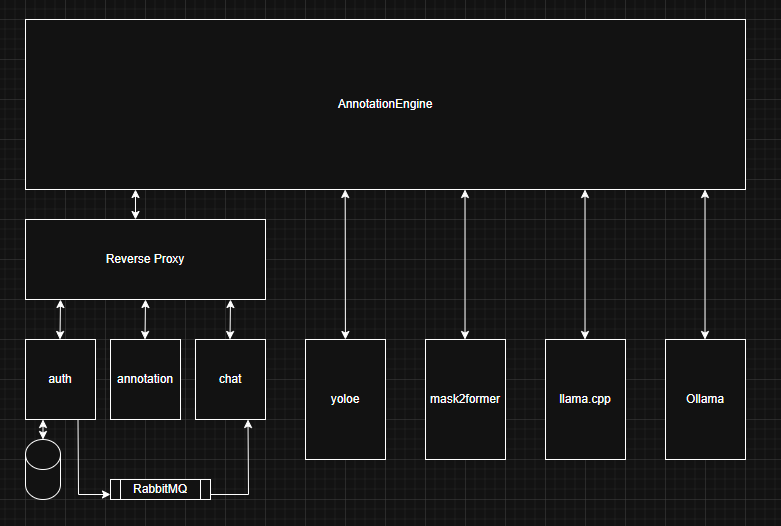
\includegraphics[width=1\textwidth,height=1\textheight,keepaspectratio]{figs/overview-of-the-project.png}
    \caption{Privire de ansamblu asupra componentelor: client desktop, modele AI locale și backend colaborativ.}
\end{figure}

\section*{Comparație funcțională}

\begin{center}
\small
\setlength{\tabcolsep}{2pt}
\begin{tabular}{|p{0.43\textwidth}|>{\centering\arraybackslash}p{0.18\textwidth}|>{\centering\arraybackslash}p{0.16\textwidth}|>{\centering\arraybackslash}p{0.16\textwidth}|}
    \hline
    \textbf{Funcționalitate} & \textbf{PyVisionAnnotator} & \textbf{CVAT} & \textbf{LabelMe (local)} \\
    \hline
    Dreptunghi / poligon & \checkmark & \checkmark & \checkmark \\
    \hline
    Măști sau contururi editabile & \checkmark & \checkmark & \checkmark \\
    \hline
    Export dataset & \checkmark & \checkmark & \checkmark \\
    \hline
    Asistență AI pentru adnotare & \checkmark & \checkmark & \checkmark \\
    \hline
    Colaborare / proiecte partajate & \checkmark & \checkmark & -- \\
    \hline
    Chat integrat & \checkmark & -- & -- \\
    \hline
    Chatbot local / LLM & \checkmark & -- & -- \\
    \hline
\end{tabular}
\end{center}

\begin{thebibliography}{4}
\footnotesize

\bibitem{cvat}
CVAT.ai contributors, \textit{CVAT: Computer Vision Annotation Tool}, GitHub repository, 2025. Disponibil: \url{https://github.com/cvat-ai/cvat}.

\bibitem{labelme}
A. Torralba, B. C. Russell și J. Yuen, ``LabelMe: Online Image Annotation and Applications,'' \textit{Proceedings of the IEEE}, vol. 98, nr. 8, pp. 1467--1484, 2010.

\bibitem{mask2former}
B. Cheng, I. Misra, A. G. Schwing, A. Kirillov și R. Girdhar, ``Masked-attention Mask Transformer for Universal Image Segmentation,'' arXiv:2112.01527, 2022.

\bibitem{yoloe}
A. Wang, L. Liu, H. Chen, Z. Lin, J. Han și G. Ding, ``YOLOE: Real-Time Seeing Anything,'' arXiv:2503.07465, 2025.
\end{thebibliography}

\end{document}
